\documentclass[border=10pt]{standalone}
\usepackage{tikz,tikz-3dplot}
\usetikzlibrary{calc,shapes,arrows,plotmarks,lindenmayersystems,decorations,decorations.markings,decorations.pathmorphing,
decorations.pathreplacing,patterns,positioning,decorations.text}
\usetikzlibrary{shadows,trees}
\usepackage{pgfplots}
\pgfplotsset{compat=1.14}

\usepackage{tkz-base,tkz-fct,tkz-euclide,tkz-tab,tkz-graph}
\usetkzobj{all}
\usetikzlibrary{spy}

\tikzset{domaine/.style 2 args={domain=#1:#2}}

\begin{document}
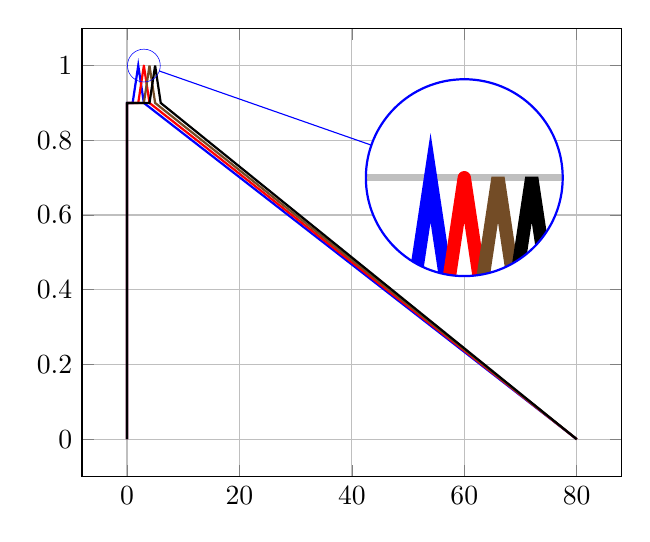
\begin{tikzpicture}[spy using outlines=
	{circle, magnification=6, connect spies}]
\begin{axis}[no markers,grid=major,
	every axis plot post/.append style={thick}]
\addplot  coordinates
 {(0, 0.0) (0, 0.9) (1, 0.9) (2, 1) (3, 0.9) (80, 0)};
\addplot +[line join=round] coordinates
 {(0, 0.0) (0, 0.9) (2, 0.9) (3, 1) (4, 0.9) (80, 0)};
\addplot +[line join=bevel] coordinates
 {(0, 0.0) (0, 0.9) (3, 0.9) (4, 1) (5, 0.9) (80, 0)};
\addplot +[miter limit=5] coordinates
 {(0, 0.0) (0, 0.9) (4, 0.9) (5, 1) (6, 0.9) (80, 0)};

  \coordinate (spypoint) at (axis cs:3,1);
  \coordinate (magnifyglass) at (axis cs:60,0.7);
\end{axis}

\spy [blue, size=2.5cm] on (spypoint)
   in node[fill=white] at (magnifyglass);
\end{tikzpicture}


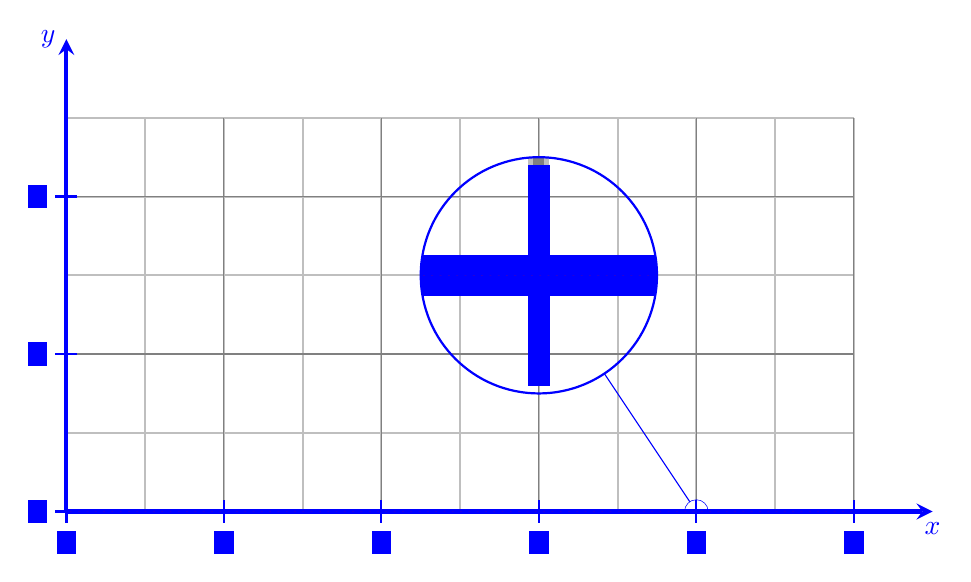
\begin{tikzpicture}[scale=2,spy using outlines={circle, magnification=10, connect spies}]
\tkzInit[xmax=5,ymax=2.5]
\tkzGrid[sub,subxstep=0.5,subystep=0.5]
\tkzAxeXY[>=stealth,color=blue,line width=1.5pt]
\tkzClip
%Courbe de la fonction
\tkzFct[color=red,samples=200,line width=1.5pt,domaine={0}{5}]
{2.5*exp(-2.5*\x)}

%Zone hachurée 1
\tkzDrawArea[pattern=north west lines,domaine={0}{1.2},pattern color=red]

%Zone hachurée 2
\tkzDrawArea[pattern=north east lines,domaine={3.5}{5},pattern color=blue]

%effet loupe
\tkzDefPoint(4,0){A}
\tkzDefPoint(3,1.5){B}
\spy [blue, size=3cm] on (A) in node (spy) at (B);

\end{tikzpicture}


\end{document}